\section{Metoda mapowania sygnału z dziedziny czasu na dziedzinę odległości}
\label{sec:Wilcox}

Opisana w poniższej sekcji metoda została zaprezentowana w artykule [\textcolor{red}{[1kasia]}]. Opiera się na odpowiednim zastosowaniu transformaty Fouriera. Pozwala na kompensację sygnału poprzez przejście z dziedziny czasu na dziedzinę odległości, dzięki czemu w wyniku otrzymywany jest skompensowany sygnał oraz informacja o długości ścieżki propagacji.

\subsection{Podstawy teoretyczne}

W niniejszej pracy rozważaną strukturą, w której powstają i propagują fale prowadzone jest długi stalowy pret. Przyjmując oznaczenie sygnału wejściowego jako $f(t)$, natomiast propagujący w pręcie sygnał jako $u(x,t)$ zakłada się iż w miejscu wzbudzenia, zachodzi zależność: 
\begin{equation}
u(x,t) = f(t)
\end{equation}
Znając $u(x,t)$ w jednym punkcie w przestrzeni oraz znając charakterystykę propagującego trybu lub trybów fali prowadzonej, można odtworzyć sygnał po dowolnej odległości propagacji oraz w dowolnym punkcie czasowym. Można to osiągnąć rozważając przesunięcie fazowe każdej składowej częstotliwości oddzielnie:
\begin{equation}
u(x,t) = \int\limits_{-\infty}^{\infty}F(\omega)e^{i(k(\omega)x - \omega t)}d\omega \label{eq:propagacja_jeden_mod}
\end{equation}
Propagacja więcej niż jednego trybu fali oznacza, iż dana częstotliwość wzbudziła więcej niż jedną jej postać. Co za tym idzie w takim przypadku również możliwe jest odtworzenie przebiegu fali poprzez lekką modyfikację wzoru \ref{eq:propagacja_jeden_mod}
\begin{equation}
u(x,t) = \int\limits_{-\infty}^{\infty}F(\omega)e^{ -i \omega t}\sum \limits _{j=1}^{n}e^{ik_j(\omega)x} d\omega\label{eq:propagacja_kilka_mod}
\end{equation}
gdzie:

$F(\omega)$ - transforamta Fouriera sygnału $f(t)$

$k_j(omega)$ - wartość j-tej liczby falowej odpowiadającej częstotliwości $\omega$

Jak już zostało wspomniane, otrzymany sygnał g(t) można odwzorować na funkcję odległości bez stosowania algorytmu komepnsacji jedynie poprzez proste odwzorowanie:
\begin{equation}
x=v_{gr}t \label{eq:x=vgrt}
\end{equation}

Gdzie $v_{gr}$ jest prędkością grupową trybu fali prowadzonej, mierzoną zazwyczaj dla częstotliwości środkowej, lub tej o największej energii. Odwzorowanie takie jest proste do osiągnięcia poprzez zwykłe skalowanie osi czasu g(t) na odległośći propagacji. W przypadku takiego odwzorowania, możliwości wykrycia defektów struktury, znajdujących się w bliskiej odległości od innych cech strukturalnych takich jak na przykład koniec badanego pręta czy punkt łączenia dwóch prętów, zależy od czasu trwania poszczególnych sygnałów. Długie sygnały będą się na siebie nakładać co może doprowadzić do niewykrycia uszkodzenia. Z tego względu sygnał g(t) powinien być jak najkrótszy. 

Przedstawiany algorytm kompensacji dyspersji, zastępuje proste mapowacznie czasu na odległość przy pomocy równania \ref{eq:x=vgrt} takim, które jest wykonywane w domenie liczby falowej. Takie podejście pozwala wziąć pod uwagę prędkości zależne od częstotliwości, czyli wzięcie pod uwagę dyspersji. Niezbędnym elementem omawianej metody jest znajomość krzywych dyspresji badanego obiektu, w zakresie propagowanych trybów. Dokładność z jaką wyliczone krzywe reprezentują rzeczywistą charakterystykę układu, znajduje odzwierciedlenie w jakości uzyskanych wyników. W sytuacji idelanej przedstawiany algorytm przywraca każdy sygnał do dokładnego kształtu pierwotnego, niezależnie od jego odległości propagacji.  

Celem omawianej metody jest przekształcenie otrzymanego sygnału $g(t)$ w funkcję odległości propagacji a nie czasu, oraz skompensowanie rozproszenia otrzymanego sygnału. Dalsze propagowanie otrzymanego sygnału zarówno w przód jak i w tył można otrzymać stosując wzór \ref{eq:propagacja_jeden_mod} lub \ref{eq:propagacja_kilka_mod}. Gdyby obliczyć kompletną mapę odległościowo czasową, sygnał propagujący dalej rozpraszałby się coraz mocniej zarówno w czasie jak i przestrzeni. Natomiast sygnał propagujący wstecz zbiegłby się do swojego minimum w pewnym punkcie, a następnie ponownie rozproszył. Minimum jego trwania przypadłoby na chwilę czasową $t=0$. Dobrze ilustruje to rysunek \ref{fig:Wilcox_propaguje}
\begin{figure}[h]
\centering
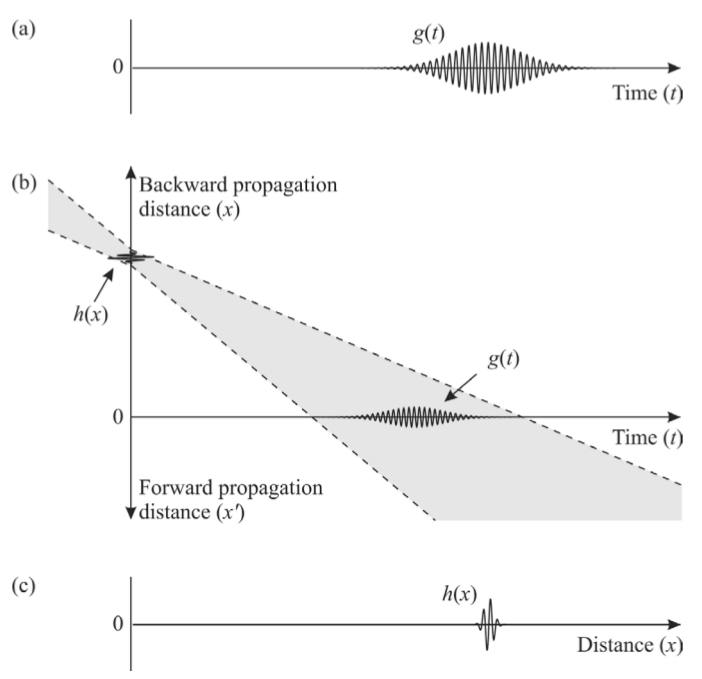
\includegraphics[width=14cm]{Zdjecia/4/Wilcox_zasada_dzial}
\caption{Zasada działania omawianej techniki kompensacji dyspersji\textcolor{red}{[1kasia]}}
\label{fig:Wilcox_propaguje}
\end{figure}
Obliczenie propagowanego wstecz sygnału dla ujemnych wartości $x'$ w $t=0$ daje dokładnie poszukiwane odwzorowanie z czasu na odlgełość propagacji, która jest poszukiwana i która kompensuje rozproszenie odebranych sygnałów. Nowa zmienna propagacji $x'$ może być zdefiniowana jako $x=-x'$. Wynika z tego, iż propagacja wsteczna może zostać opisana wzorem:

\begin{equation}
h(x) = u(-x',0) = \int \limits_{-\infty}^{\infty}G(\omega)e^{-ik(\omega)x}d\omega \label{eq:wsteczna propagacja}
\end{equation}

gdzie:

$G(\omega)$ - transformata Fouriera odebranego sygnału w dziedzinie czasu $g(t)$

$h(x)$ - skompensowany dyspersyjnie przebieg odległości.

Funkja h(x) przedstawiona jest na rysunku \ref{fig:Wilcox_propaguje} (c).

W niniejszej pracy nie został uwzględniony współczynnik odbicia $A_j$. Na potrzeby symulacji przyjęte zostało iż jest on stały, niezależny od czestotliwości i wynosi 1. Gdyby jednak brać go pod uwagę to wzór 4.16 przyjałby postać:
\begin{equation}
g(t) = \sum \limits _{j}\int\limits_{-\infty}^{\infty}A_j(\omega)F(\omega)e^(ik(\omega)x_j-wt)d\omega
\end{equation}

W przyadku stałego współczynnika odbić wszystkie sygnały w h(x) powinny mieć ten sam kształt obwiedni co oryginalny sygnał wejściowy. Gdyby jednak zależał on od częstotliwości , wówczas obwiednia sygnału w h(x) zostanie zniekształcona i na ogół wydłużona. Takie zniekształcenie jest artefaktem charakterystycznym dla danego punktu odbicia fali. Co za tym idzie takie zakłócenie byłoby obserwowane nawet, gdyby zjawisko dyspersji nie występowało. 

\subsection{implementacja numeryczna}
Równanie \ref{eq:wsteczna propagacja} jest podstawowym równaniem omawianej metody. Jest równaniem kompensacji dyspersji dla funkcji ciągłych. W praktyce sygnał g(t) nie jest sygnałem ciągłym a sygnałem dyskretnym, wygenerowanym w aplikacji lub otrzymanym z przetwornika. Na potrzeby tego rozdziału przyjmijmy nastepujące oznaczenia:

$m$ - liczna próbek sygnału g(t)

$\Delta t$ - okres próbkowania sygnało g(t)

$m\Delta t$ - całkowity czas trwania sygnału g(t)

$n$ - liczba próbek otrzymanego sygnału w dziedzinie odległośći h(x)

$\Delta x$ -przestrzenny okres próbkowania h(x)

$n\Delta x$ - całkowita przestrzenna długość sygnału

Najprostszą implementacją omawianego algorytmu jest poddanie sygnału g(t) szybkiej transformacie Fouriera, a następnie całkowanie numeryczne w zakresie częstotliwości sygnału wejściowego. Takie rozwiązanie byłoby niezwykle czasochłonne ponieważ całkowanie musiałoby zostać wykonane dla każdego z n punkót w skompensowanym sygnale h(x). Metodą, która została zaimplementowana w opisanej aplikacji polega na modyfikacji równania \ref{eq:wsteczna propagacja}. Ta zmiana pozwala na wykonywanie całkowania w ramach algorytmu odwrotnej transformaty Fouriera. Skompensowany sygnał jest funkcją odległości. Odwrotna transformata Fouriera musi zostać zastosowana na sygnale w dziedzinie liczby falowej. Wynika z tego, iż zmienna całkowania w równaniu \ref{eq:wsteczna propagacja} musi zostać zmieniona z $\omega$ na $k$. Można to łatwo zrobić używając poniższych zależności:
\begin{equation}
d\omega = v_{gr}(\omega)dk
\end{equation}
\begin{equation}
\omega = v_{ph}(\omega)k
\end{equation}

Gdzie:

$v_{gr}(\omega)$ - prędkość grupowa propagującej postaci

$v_{ph}(\omega)$ - prędkość fazowa propagującej postaci

Biorąc to pod uwagę równanie \ref{eq:wsteczna propagacja} można zapisać jako:


\begin{equation}
h(x) = \int\limits_{-\infty}^{infty}H(k)e^{-ikx}dk \label{eq:h(x) dobre}
\end{equation}

\begin{equation}
H(k) = G(k)v_gr(k)
\end{equation}

$$
\omega = \omega(k)
$$

Równanie \ref{eq:h(x) dobre} ma postać odwrotnej transformaty Fouriera $H(k)$, w punktach spróbkowanych ze stałym przestrzennym okresem próbkowania $\Delta k$. Uzyskana z transformaty Fouriera funkcja $G(\omega)$ jest funkcją o punktach równomiernie spróbkowanych w dziedzinie częstotliwości. Ze względu na nieliniowy charakter krzywych dyspersji przejście z dziedziny częstości na dziedzinę liczby falowej dałoby w rezultacie funkcję o nierównomiernie spróbkowanej osi k. Aby uzyskać porządany efekt konieczne jest użycie znanej z krzywej dyspersji zależności między wartościami $\omega$ oraz $k$, aby interpolować funkcję G, tak by znaleźć jej wartości w punktach równomiernie rozmieszczonych w dziedzinie liczby falowej.

$G(\omega)$ jest sygnałem zawierającym informacje zarówno o fazie jak i amplitudzie sygnału. W rozwiązaniu numerycznym istotne jest aby dobrać odpowiednie wartości kroków. Zbyt duże ich wartości mogą spowodować utratę informacji, natomiast zbyt małe prowadzą do znacznego wydłużania czasu obliczeń, w zamian za co uzyskiwane wyniki są dokładniejsze i wpływ szumu staje się mniej znaczący. W celu zmniejszenia szumu powodowanego przez błędy interpolacji w końcowym, skompensowanym sygnale, otrzymany sygnał g(t) wypełnia się zerami.W aplikacji użytkownik ma możliwość samodzielnie podać ile razy chce wydłużyć sygnał poprzez wypełnienie zerami. Ograniczenim podlega zarówno $\Delta k$ jak i ilość punktów liczb falowych n. Aby zapobiec zawijaniu sygnału w domenie odległości, minimalna długość skompensowanego sygnału h(x) musi być większa od długości pierwotnego sygnału g(t) pomnożonego przez maksymalną prędkość grupową $v_{max}$.
\begin{equation}
n\Delta x > m\Delta tv_{max}\label{eq:nierownosc dlugosci sygnalow}
\end{equation} 

Powyższa nierówność określa nam maksymalny rozmiar kroku liczby falowej jako:

\begin{equation}
\Delta k = \frac{1}{n\Delta x} < \frac{1}{ m\Delta tv_{max}}\label{eq:nierown delta k}
\end{equation}

Aby cała energia pierwotnego sygnału została poprawnie odwzorowana na dziedzinę odległości, liczba falowa Nyquista $k_{Nyq}$ musi być większa lub równa liczbie falowej trybu fali prowadzonej o częstotliwości Nyquista $f_{Nyq}$ oryginalnego sygnału. Co można zapisać jako:
\begin{equation}
k_{Nyq}\geq k(f_{Nyq})\label{eq:k Nyquista}
\end{equation}
$$
\geq k(\frac{1}{2\Delta t})
$$

Nierówność \ref{eq:k Nyquista} oraz równanie \ref{eq:nierown delta k} pozwalają określić minimalną liczbę punktów w sygnale h(x)
\begin{equation}
n > 2\frac{k_{Nyq}}{\Delta k}
\end{equation}

W zaimplementowanym algorytmie, pierwszym krokiem jest wydłużenie otrzymanego sygnału zadaną ilość razy oraz wykonanie szybkiej transformaty Fouriera na wydłużonym sygnale. Następnie na podstawie przedstawionych ograniczeń dobierana jest wartość kroku $\Delta k$ oraz obliczana wartość $k_{max} = k(\omega _{max})$. Znając te parametry tworzony jest wektor zawierający równomiernie rozłożone wartości liczby falowej. Przy użyciu krzywej dyspersji, interpolując liniowo potrzebne wartości obliczana jest funkcja $G(k)$ oraz $v_{gr}(k)$ w tych samych punktach. Następnie wyliczana zostaje funkcja $H(k)$ mająca równomiernie rozłożone wartości liczby falowej. Ostatnim etapem jest zastosowanie szybkiej odwrotnej transformaty Fouriera co pozwala uzyskać poszukiwany sygnał h(x).

W przypadku gdy mamy do czynienia z propagacją większej ilości postaci fal lub gdy podczas odbicia następuje konwersja trybu fali prowadzonej dokonywane jest uśrednianie propagowanych postaci. Przy założeniu, że propagują jednocześnie dwie postacie równanie \ref{eq:wsteczna propagacja} można ponownie zapisać jako:
\begin{equation}
h(x) = \int\limits _{-\infty}^{\infty}G(\omega)e^{i(k_1(\omega)+k_2(\omega))\frac{x}{2}}d\omega \label{eq:wiele postaci}
\end{equation}
W implementacji oznacza to, iż kilka krzywych dyspersji zostaje ośrednionych do jednej postaci w której $k_{12} = \frac{1}{2}(k_1(\omega) + k_2(\omega))$
\subsection{Wybrane wyniki symulacji}
Przykładowe sygnał wejściowy wygenerowane w aplikacji zaprezentowane zostały na rysunku \ref{fig:przykl_we}.
\begin{figure}[h]
\centering
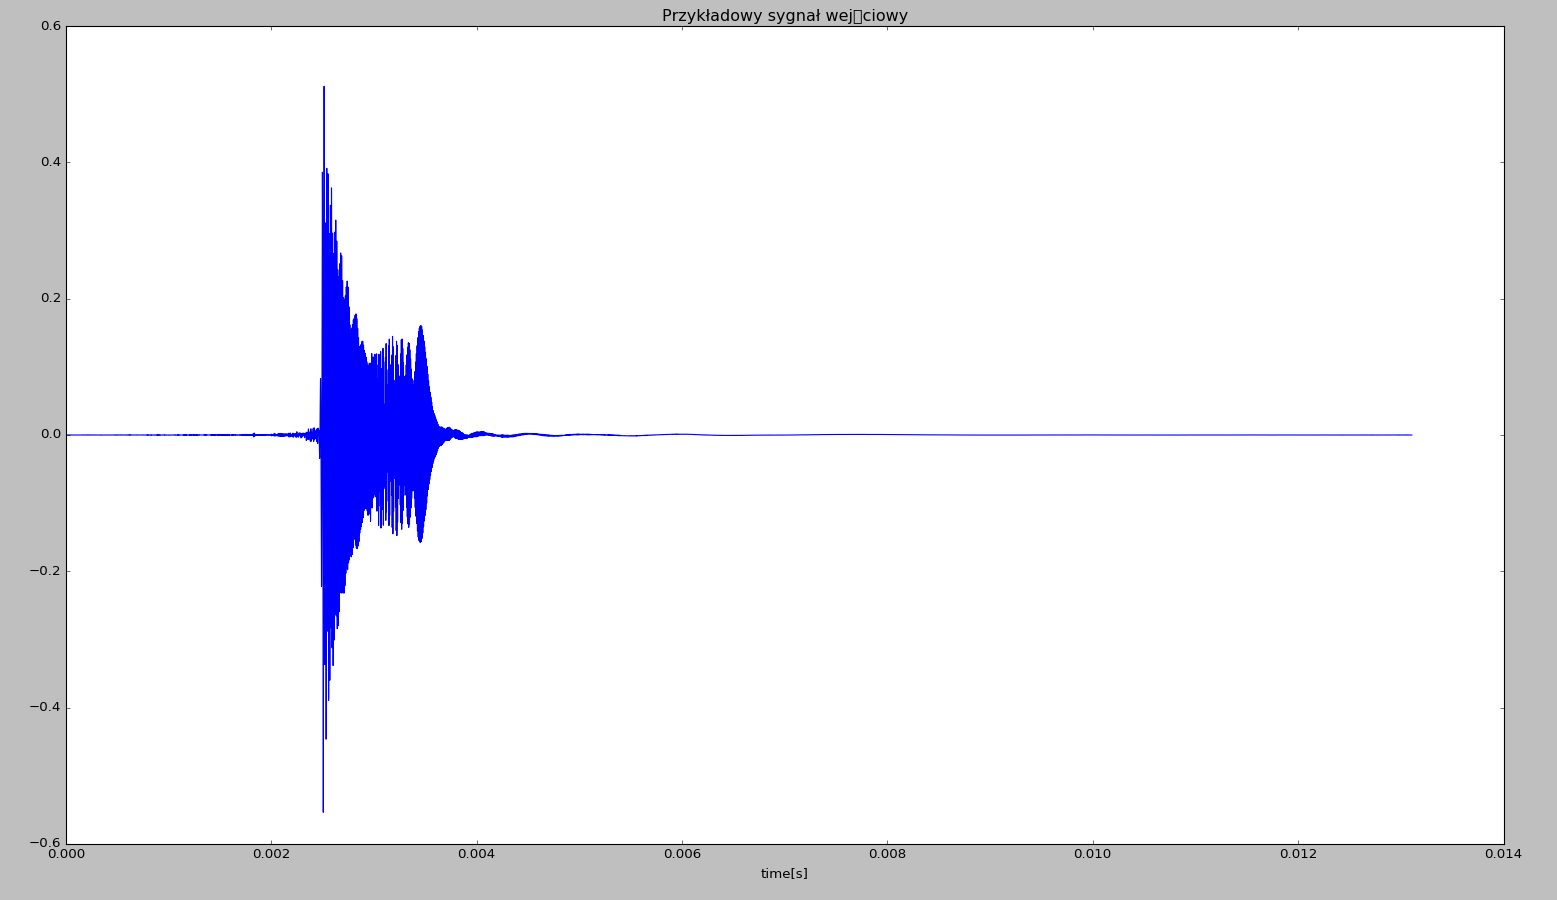
\includegraphics[width=14cm]{Zdjecia/4/przykl_we}
\caption{przykładowy sygnał wejściowy}
\label{fig:przykl_we}
\end{figure}
Przykładowa krzywa dyspersji powstała w wyniku uśrednienia trzech pierwszych postaci fali zaprezentowana została na rysunku \ref{fig:mean}. 
\begin{figure}[h]
\centering
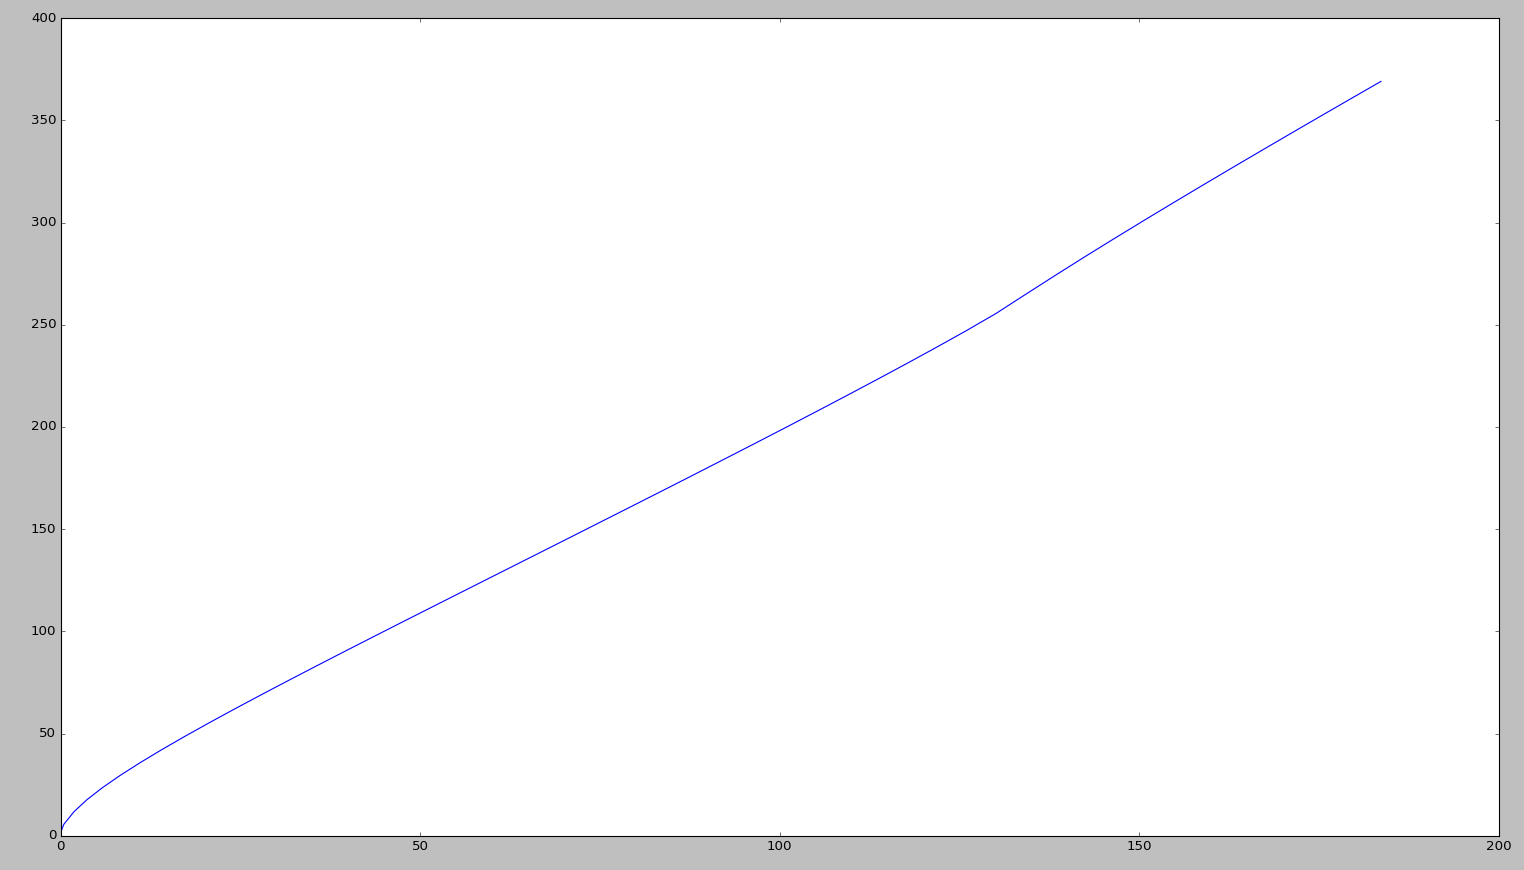
\includegraphics[width=14cm]{Zdjecia/4/meanmode}
\caption{Średnia krzywa dyspersji powstała z uśrednienia trzech pierwszych krzywych}
\label{fig:mean}
\end{figure}
Na kolejnym rysunku \ref{fig:wil1} przedstawiono porównanie sygnału przed i po kompensacji. Rozproszony sygnał został skompensowany do znacznie krótszej postaci. Dodatkowo w łatwy sposób możliwe jest odczytanie długości ścieżki propagacji, która w tym przypadku wynosiła dwa metry. 
\begin{figure}[h]
\centering
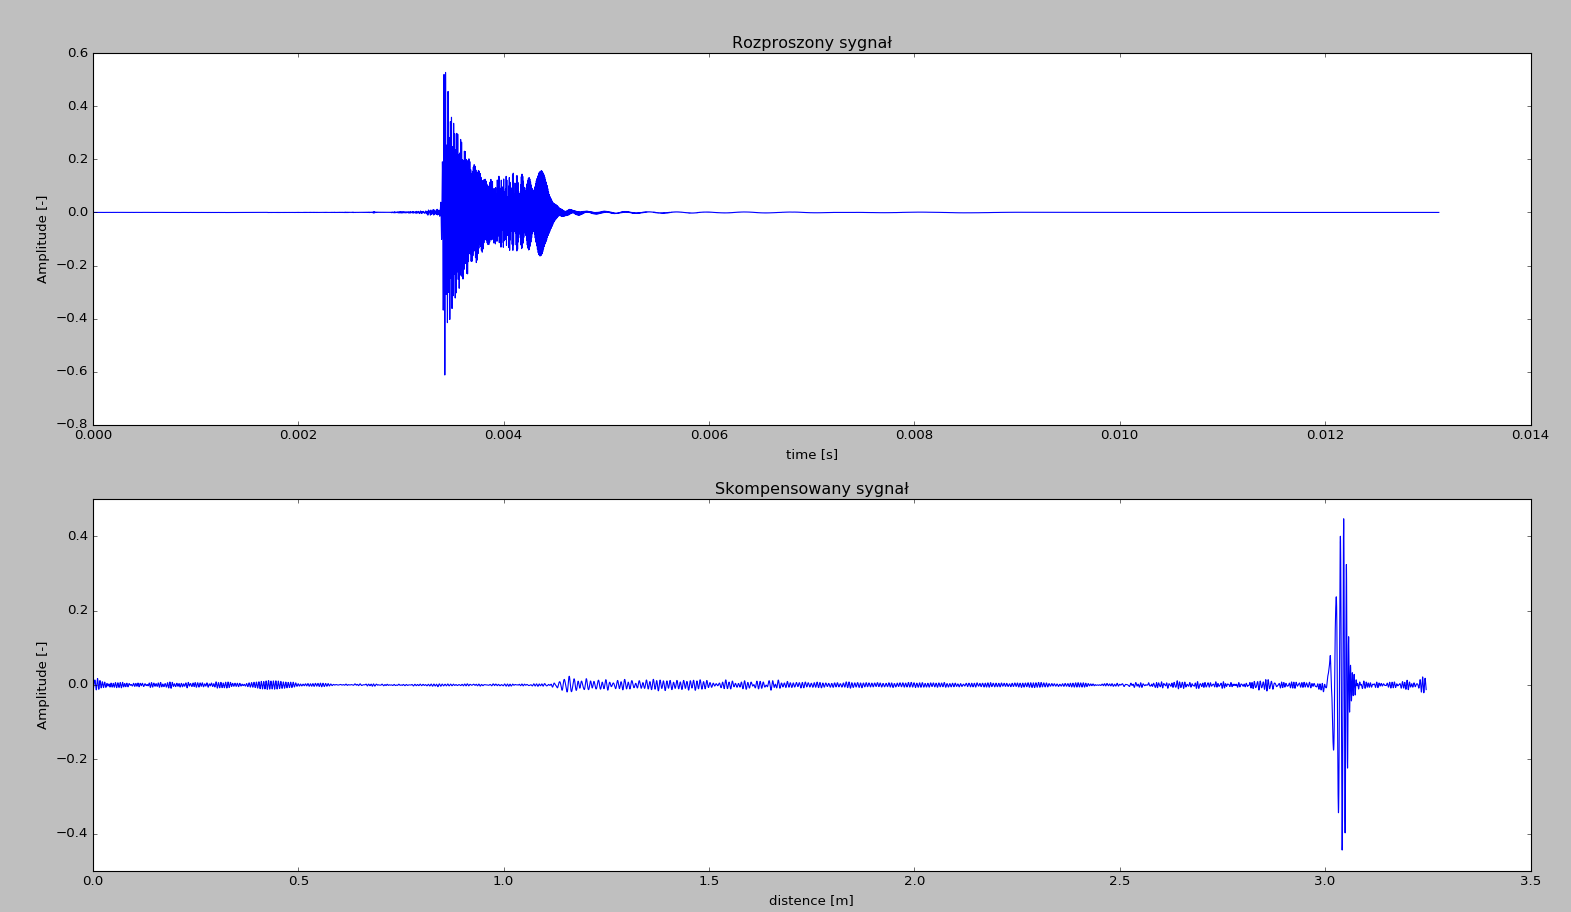
\includegraphics[width=14cm]{Zdjecia/4/wilcox1}
\caption{Porównanie sygnału przed i po kompensacji}
\label{fig:wil1}
\end{figure}
Kolejny rysunek przedstawia wyniki symulacji, w której sygnał nie został dostatecznie wydłużony w wyniku czego otrzymany wynik był nieczytelny \ref{fig:zawij}
\begin{figure}[h]
\centering
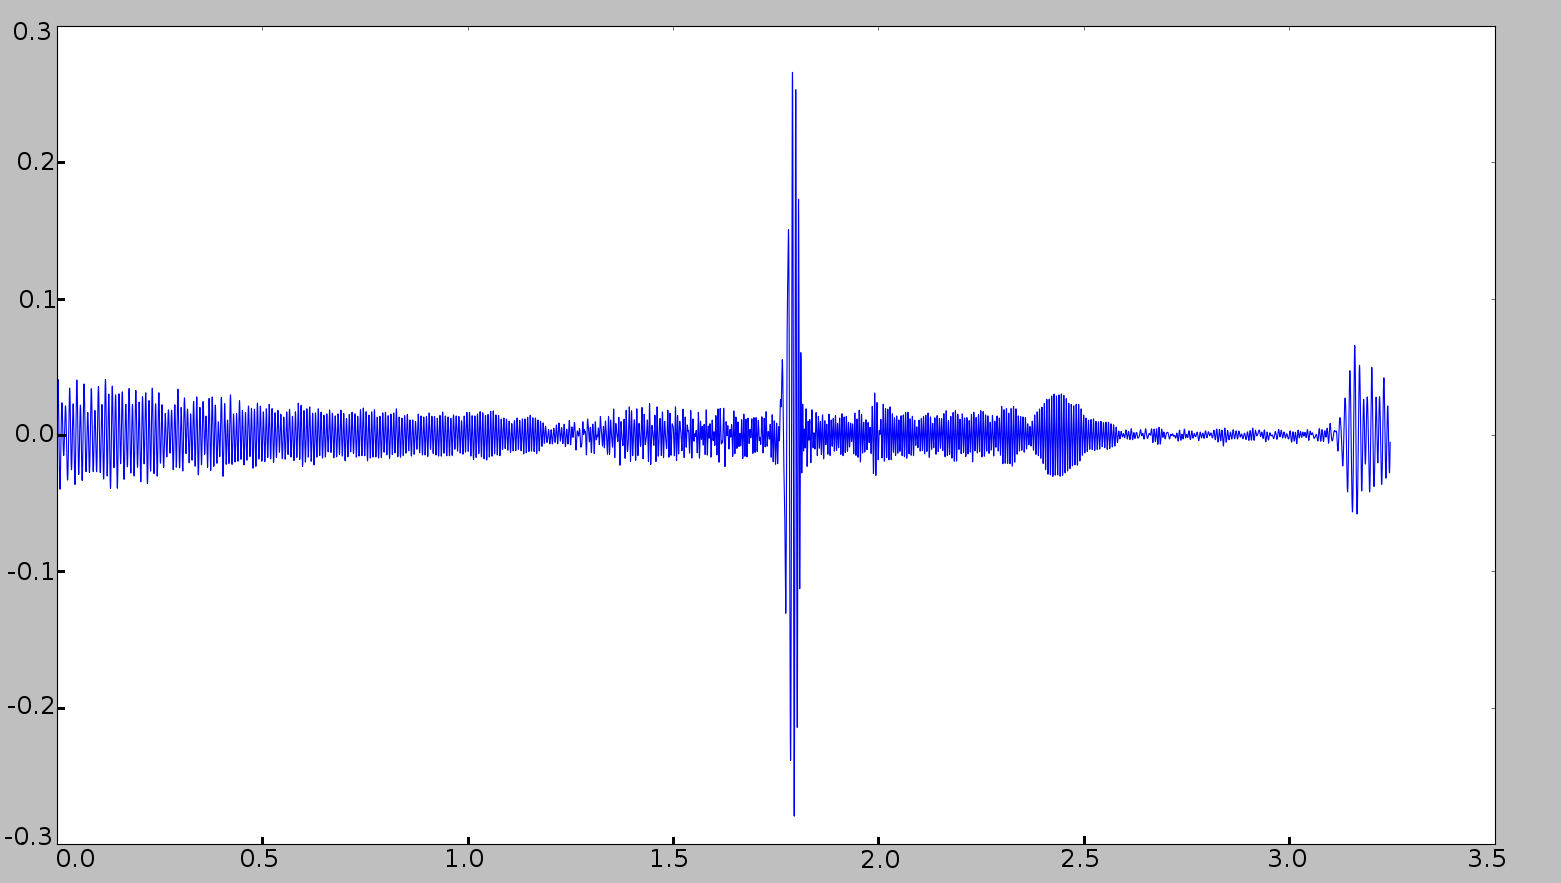
\includegraphics[width=14cm]{Zdjecia/4/naklada}
\caption{Sygnał, który przepropagował 5 metrów, widoczne zawijanie sygnału}
\label{fig:zawij}
\end{figure}
Ostatni rysunek prezentuje porównanie skompensowanego sygnału z sygnałem wejściowym, w przypadku, gdy symulowana była propagacja pierwszych trzech postaci fali prowadzonej. Omawiana metoda daje najlepsze wyniki kompensacji. Ze wszystkich prezentowanych w ramach niniejszej pracy metod, ta najdokładniej odwzorowuje zadany na wejściu sygnał. Jej kolejnymi atutami są minimalne wymagania jeśli chodzi o dane wejściowe oraz największa ilość otrzymywanych informacji. Na podstawie znajomości jedynie przepropagowanego sygnału oraz znajomości krzywych dyspersji propagujących postaci jest ona w stanie skompensować rozproszony sygnał, podając jednocześnie informację o długości ścieżki propagacji. Algorytm radzi sobie dobrze zarówno z kompensacją jednej propagującej postaci jak i dwiema a nawet trzema.

\begin{figure}[h]
\centering
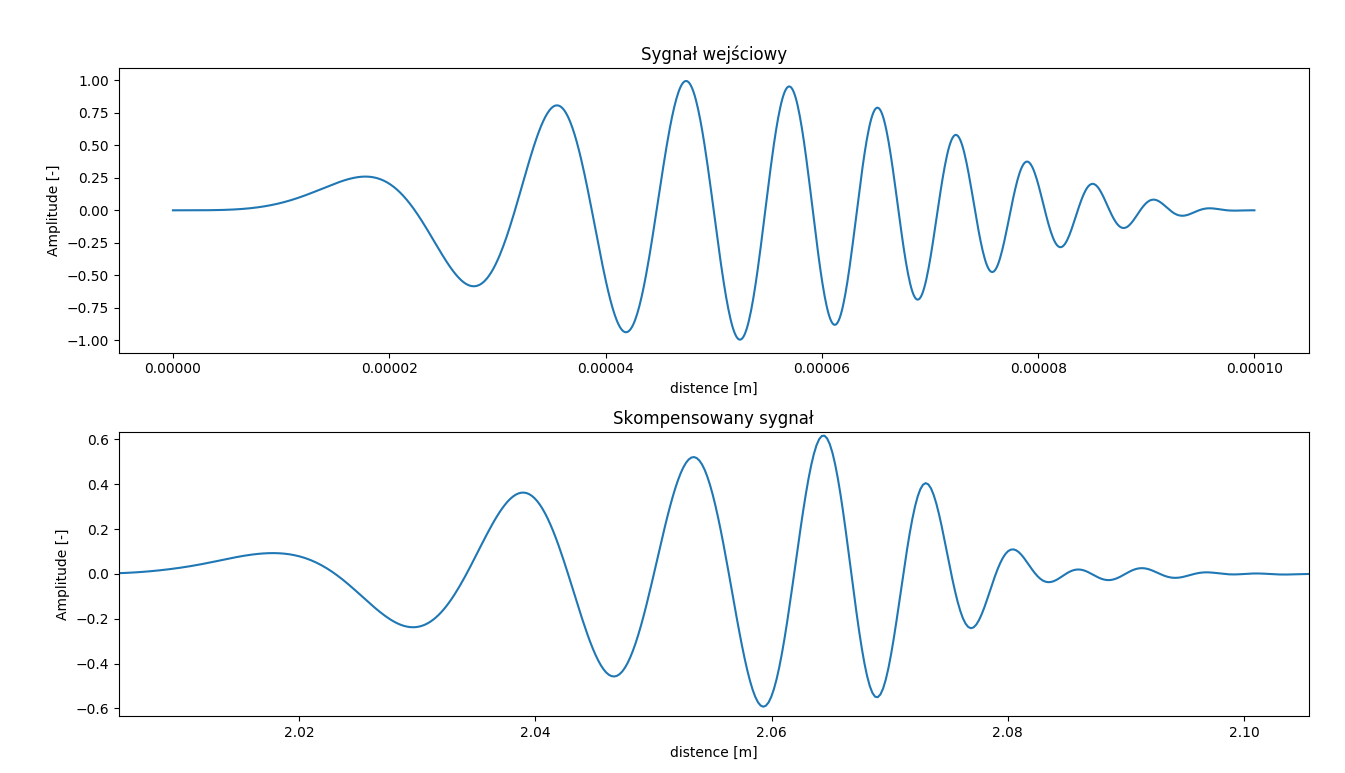
\includegraphics[width=14cm]{Zdjecia/4/Wilcoxporownanie}
\caption{Porównanie sygnału wejściowego oraz sygnału skompensowanego}
\label{fig:willast}
\end{figure}